% Options for packages loaded elsewhere
\PassOptionsToPackage{unicode}{hyperref}
\PassOptionsToPackage{hyphens}{url}
%
\documentclass[onecolumn]{article}
\usepackage{lmodern}
\usepackage{amssymb,amsmath}
\usepackage{ifxetex,ifluatex}
\ifnum 0\ifxetex 1\fi\ifluatex 1\fi=0 % if pdftex
  \usepackage[T1]{fontenc}
  \usepackage[utf8]{inputenc}
  \usepackage{textcomp} % provide euro and other symbols
\else % if luatex or xetex
  \usepackage{unicode-math}
  \defaultfontfeatures{Scale=MatchLowercase}
  \defaultfontfeatures[\rmfamily]{Ligatures=TeX,Scale=1}
\fi
% Use upquote if available, for straight quotes in verbatim environments
\IfFileExists{upquote.sty}{\usepackage{upquote}}{}
\IfFileExists{microtype.sty}{% use microtype if available
  \usepackage[]{microtype}
  \UseMicrotypeSet[protrusion]{basicmath} % disable protrusion for tt fonts
}{}
\makeatletter
\@ifundefined{KOMAClassName}{% if non-KOMA class
  \IfFileExists{parskip.sty}{%
    \usepackage{parskip}
  }{% else
    \setlength{\parindent}{0pt}
    \setlength{\parskip}{6pt plus 2pt minus 1pt}}
}{% if KOMA class
  \KOMAoptions{parskip=half}}
\makeatother
\usepackage{xcolor}
\IfFileExists{xurl.sty}{\usepackage{xurl}}{} % add URL line breaks if available
\IfFileExists{bookmark.sty}{\usepackage{bookmark}}{\usepackage{hyperref}}
\hypersetup{
  pdftitle={Trabajo práctico N°2: Razonamiento},
  pdfauthor={Gino Avanzini; Emiliano Cabrino; Adrián Cantaloube; Gonzalo Fernández},
  hidelinks,
  pdfcreator={LaTeX via pandoc}}
\urlstyle{same} % disable monospaced font for URLs
\usepackage{color}
\usepackage{fancyvrb}
\newcommand{\VerbBar}{|}
\newcommand{\VERB}{\Verb[commandchars=\\\{\}]}
\DefineVerbatimEnvironment{Highlighting}{Verbatim}{commandchars=\\\{\}}
% Add ',fontsize=\small' for more characters per line
\newenvironment{Shaded}{}{}
\newcommand{\AlertTok}[1]{\textcolor[rgb]{1.00,0.00,0.00}{\textbf{#1}}}
\newcommand{\AnnotationTok}[1]{\textcolor[rgb]{0.38,0.63,0.69}{\textbf{\textit{#1}}}}
\newcommand{\AttributeTok}[1]{\textcolor[rgb]{0.49,0.56,0.16}{#1}}
\newcommand{\BaseNTok}[1]{\textcolor[rgb]{0.25,0.63,0.44}{#1}}
\newcommand{\BuiltInTok}[1]{#1}
\newcommand{\CharTok}[1]{\textcolor[rgb]{0.25,0.44,0.63}{#1}}
\newcommand{\CommentTok}[1]{\textcolor[rgb]{0.38,0.63,0.69}{\textit{#1}}}
\newcommand{\CommentVarTok}[1]{\textcolor[rgb]{0.38,0.63,0.69}{\textbf{\textit{#1}}}}
\newcommand{\ConstantTok}[1]{\textcolor[rgb]{0.53,0.00,0.00}{#1}}
\newcommand{\ControlFlowTok}[1]{\textcolor[rgb]{0.00,0.44,0.13}{\textbf{#1}}}
\newcommand{\DataTypeTok}[1]{\textcolor[rgb]{0.56,0.13,0.00}{#1}}
\newcommand{\DecValTok}[1]{\textcolor[rgb]{0.25,0.63,0.44}{#1}}
\newcommand{\DocumentationTok}[1]{\textcolor[rgb]{0.73,0.13,0.13}{\textit{#1}}}
\newcommand{\ErrorTok}[1]{\textcolor[rgb]{1.00,0.00,0.00}{\textbf{#1}}}
\newcommand{\ExtensionTok}[1]{#1}
\newcommand{\FloatTok}[1]{\textcolor[rgb]{0.25,0.63,0.44}{#1}}
\newcommand{\FunctionTok}[1]{\textcolor[rgb]{0.02,0.16,0.49}{#1}}
\newcommand{\ImportTok}[1]{#1}
\newcommand{\InformationTok}[1]{\textcolor[rgb]{0.38,0.63,0.69}{\textbf{\textit{#1}}}}
\newcommand{\KeywordTok}[1]{\textcolor[rgb]{0.00,0.44,0.13}{\textbf{#1}}}
\newcommand{\NormalTok}[1]{#1}
\newcommand{\OperatorTok}[1]{\textcolor[rgb]{0.40,0.40,0.40}{#1}}
\newcommand{\OtherTok}[1]{\textcolor[rgb]{0.00,0.44,0.13}{#1}}
\newcommand{\PreprocessorTok}[1]{\textcolor[rgb]{0.74,0.48,0.00}{#1}}
\newcommand{\RegionMarkerTok}[1]{#1}
\newcommand{\SpecialCharTok}[1]{\textcolor[rgb]{0.25,0.44,0.63}{#1}}
\newcommand{\SpecialStringTok}[1]{\textcolor[rgb]{0.73,0.40,0.53}{#1}}
\newcommand{\StringTok}[1]{\textcolor[rgb]{0.25,0.44,0.63}{#1}}
\newcommand{\VariableTok}[1]{\textcolor[rgb]{0.10,0.09,0.49}{#1}}
\newcommand{\VerbatimStringTok}[1]{\textcolor[rgb]{0.25,0.44,0.63}{#1}}
\newcommand{\WarningTok}[1]{\textcolor[rgb]{0.38,0.63,0.69}{\textbf{\textit{#1}}}}
\usepackage{graphicx,grffile}
\makeatletter
\def\maxwidth{\ifdim\Gin@nat@width>\linewidth\linewidth\else\Gin@nat@width\fi}
\def\maxheight{\ifdim\Gin@nat@height>\textheight\textheight\else\Gin@nat@height\fi}
\makeatother
% Scale images if necessary, so that they will not overflow the page
% margins by default, and it is still possible to overwrite the defaults
% using explicit options in \includegraphics[width, height, ...]{}
\setkeys{Gin}{width=\maxwidth,height=\maxheight,keepaspectratio}
% Set default figure placement to htbp
\makeatletter
\def\fps@figure{htbp}
\makeatother
\setlength{\emergencystretch}{3em} % prevent overfull lines
\providecommand{\tightlist}{%
  \setlength{\itemsep}{0pt}\setlength{\parskip}{0pt}}
\setcounter{secnumdepth}{-\maxdimen} % remove section numbering

\title{Trabajo práctico N°2: Razonamiento}
\author{Gino Avanzini \and Emiliano Cabrino \and Adrián Cantaloube \and Gonzalo Fernández}
\date{Mayo de 2019}

\begin{document}
\maketitle

\hypertarget{desarrollo-y-anuxe1lisis-de-una-base-de-conocimiento-para-una-planta-de-reducciuxf3n-de-presiuxf3n-de-gas}{%
\section{Desarrollo y análisis de una base de conocimiento para una
planta de reducción de presión de
gas}\label{desarrollo-y-anuxe1lisis-de-una-base-de-conocimiento-para-una-planta-de-reducciuxf3n-de-presiuxf3n-de-gas}}

Utilizamos el lenguaje Prolog para generar la base de conocimientos
según los lineamientos de la gráfica de acción de la planta.

De forma sencilla, en el archivo ``ejercicio1bis.pl'' ingresamos las
reglas axiomáticas y los ground facts. Las primeras las escribimos de
tal manera que Prolog acceda a su algoritmo interno de backtracking
permitiendo verificar, primero si el estado en el que nos encontramos
analizando es válido, para luego buscar el axioma superior a él (de
cumplirse la condición) y verificar el nuevo estado para saber si
detenerse y entregar la orden o continuar buscando de forma automática.
Los estados se podrán modificar dinamicamente utilizando los comandos
assert y retract, modificándolos según lo que ocurra en la planta. Una
vez cerrado el programa estos cambios en las condiciones de los estados
se perderán.

Se presentó una variante de este problema (el archivo ``ejercicio1.pl'')
sin el uso del backtracking en donde el usuario puede acceder a
cualquier parte del árbol formulando la pregunta e indicando si esta es
verdadera o falsa según lo que suceda en la planta. El programa le dirá
que acción tomar. Esto puede ser o una orden o que se verifique otro
axioma. Aquí no serán necesarios los comandos assert y retract ya que
los estados se han indicado como variables que el usuario debe ingresar
al hacer la pregunta, o sea, que no forman parte de los ground facts. En
este enfoque también se agregaron valores de variables como thickness o
max regulating pressure para distintos tipos de válvulas (sv y rv) como
se sugiere en el enunciado del ejercicio.

Además se realizó otro ejercicio con el uso del árbol de decisión para
tratamiento médico ante la inhalación de fosgeno\footnote{\href{https://www.americanchemistry.com/Phosgene/Medical-Treatment-Decision-Tree-for-Medical-Professionals.html}{PHOSGENE:
  Information on Options for First Aid and Medical Treatment}, American
  Chemistry Council.}. La base de conocimiento se encuentra en el
archivo \emph{treatment.pl}

\begin{figure}
\centering
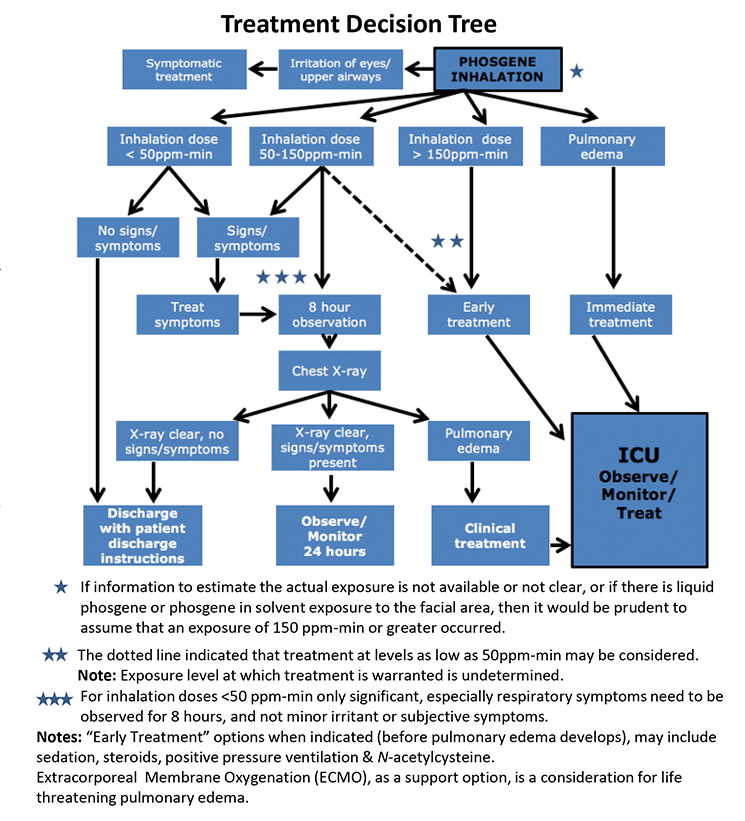
\includegraphics{treatment_decision_tree.png}
\caption{Árbol de decisión para tratamiento por inhalación de fosgeno}
\end{figure}

\hypertarget{implementaciuxf3n-de-un-sistema-de-inferencia-difusa-para-controlar-un-puxe9ndulo-invertido}{%
\section{Implementación de un sistema de inferencia difusa para
controlar un péndulo
invertido}\label{implementaciuxf3n-de-un-sistema-de-inferencia-difusa-para-controlar-un-puxe9ndulo-invertido}}

\hypertarget{anuxe1lisis-del-modelo-fuxedsico-del-puxe9ndulo-invertido}{%
\subsection{Análisis del modelo físico del péndulo
invertido}\label{anuxe1lisis-del-modelo-fuxedsico-del-puxe9ndulo-invertido}}

Las constantes del modelo físico son las siguientes:

\begin{Shaded}
\begin{Highlighting}[]
\ImportTok{from}\NormalTok{ math }\ImportTok{import}\NormalTok{ sin, cos, }\BuiltInTok{pow}\NormalTok{, pi}

\CommentTok{#--------------------------------------------------}
\CommentTok{# Constantes del modelo}
\CommentTok{#--------------------------------------------------}
\NormalTok{g }\OperatorTok{=} \FloatTok{9.81}    \CommentTok{# [m/s^2]   Aceleración de la gravedad}
\NormalTok{F }\OperatorTok{=} \DecValTok{0}       \CommentTok{# [N]       Fuerza externa}
\NormalTok{m }\OperatorTok{=} \FloatTok{0.2}     \CommentTok{# [Kg]      Masa del péndulo}
\NormalTok{l }\OperatorTok{=} \FloatTok{0.5}     \CommentTok{# [m]       Longitud del péndulo}
\NormalTok{M }\OperatorTok{=} \DecValTok{2}       \CommentTok{# [Kg]      Masa del carro}
\CommentTok{#--------------------------------------------------}
\end{Highlighting}
\end{Shaded}

A continuación se calcula el modelo en el tiempo, sin aplicar ningún
tipo de control:

\begin{Shaded}
\begin{Highlighting}[]
\KeywordTok{def}\NormalTok{ update(x, dt, F):}

\NormalTok{    x_t }\OperatorTok{=}\NormalTok{ x}

\NormalTok{    num }\OperatorTok{=}\NormalTok{ g }\OperatorTok{*}\NormalTok{ sin(x[}\DecValTok{0}\NormalTok{]) }\OperatorTok{+}\NormalTok{ cos(x[}\DecValTok{0}\NormalTok{]) }\OperatorTok{*}\NormalTok{ (}\OperatorTok{-}\NormalTok{ F }\OperatorTok{-}\NormalTok{ m }\OperatorTok{*}\NormalTok{ l }\OperatorTok{*} \BuiltInTok{pow}\NormalTok{(x[}\DecValTok{1}\NormalTok{], }\DecValTok{2}\NormalTok{) }\OperatorTok{*}\NormalTok{ sin(x[}\DecValTok{0}\NormalTok{])) }\OperatorTok{/}\NormalTok{ (M }\OperatorTok{+}\NormalTok{ m)}
\NormalTok{    den }\OperatorTok{=}\NormalTok{ l }\OperatorTok{*}\NormalTok{ (}\DecValTok{4}\OperatorTok{/}\DecValTok{3} \OperatorTok{-}\NormalTok{ m }\OperatorTok{*} \BuiltInTok{pow}\NormalTok{(cos(x[}\DecValTok{0}\NormalTok{]), }\DecValTok{2}\NormalTok{) }\OperatorTok{/}\NormalTok{ (M }\OperatorTok{+}\NormalTok{ m))}

\NormalTok{    x_t[}\DecValTok{2}\NormalTok{] }\OperatorTok{=}\NormalTok{ num }\OperatorTok{/}\NormalTok{ den}

\NormalTok{    x_t[}\DecValTok{1}\NormalTok{] }\OperatorTok{=}\NormalTok{ x[}\DecValTok{1}\NormalTok{] }\OperatorTok{+}\NormalTok{ x[}\DecValTok{2}\NormalTok{]}\OperatorTok{*}\NormalTok{dt}
\NormalTok{    x_t[}\DecValTok{0}\NormalTok{] }\OperatorTok{=}\NormalTok{ x[}\DecValTok{0}\NormalTok{] }\OperatorTok{+}\NormalTok{ x[}\DecValTok{1}\NormalTok{]}\OperatorTok{*}\NormalTok{dt }\OperatorTok{+}\NormalTok{ x[}\DecValTok{2}\NormalTok{]}\OperatorTok{*}\BuiltInTok{pow}\NormalTok{(dt, }\DecValTok{2}\NormalTok{)}\OperatorTok{/}\DecValTok{2}

    \ControlFlowTok{return}\NormalTok{ x_t}
\end{Highlighting}
\end{Shaded}

\begin{Shaded}
\begin{Highlighting}[]
\NormalTok{MAX_ITER }\OperatorTok{=} \DecValTok{2000}

\NormalTok{dt }\OperatorTok{=} \FloatTok{0.001}
\NormalTok{t }\OperatorTok{=} \DecValTok{0}

\NormalTok{x }\OperatorTok{=}\NormalTok{ [}\OperatorTok{-}\NormalTok{pi }\OperatorTok{+} \FloatTok{0.01}\NormalTok{, }\DecValTok{0}\NormalTok{, }\DecValTok{0}\NormalTok{]}

\NormalTok{pos }\OperatorTok{=}\NormalTok{ []}
\NormalTok{vel }\OperatorTok{=}\NormalTok{ []}
\NormalTok{acel }\OperatorTok{=}\NormalTok{ []}
\NormalTok{time }\OperatorTok{=}\NormalTok{ []}

\ControlFlowTok{while}\NormalTok{(t }\OperatorTok{<}\NormalTok{ MAX_ITER):}

\NormalTok{    pos.append(x[}\DecValTok{0}\NormalTok{])}
\NormalTok{    vel.append(x[}\DecValTok{1}\NormalTok{])}
\NormalTok{    acel.append(x[}\DecValTok{2}\NormalTok{])}

\NormalTok{    x }\OperatorTok{=}\NormalTok{ update(x, dt, }\DecValTok{0}\NormalTok{)}

\NormalTok{    time.append(t)}

\NormalTok{    t }\OperatorTok{+=}\NormalTok{ dt}
\end{Highlighting}
\end{Shaded}

Las gráficas de ángulo \(\theta\), velocidad angular y aceleración
angular en el tiempo son:

\begin{Shaded}
\begin{Highlighting}[]
\ImportTok{from}\NormalTok{ matplotlib }\ImportTok{import}\NormalTok{ pyplot }\ImportTok{as}\NormalTok{ plt}

\NormalTok{fig, (ax0, ax1, ax2) }\OperatorTok{=}\NormalTok{ plt.subplots(}\DecValTok{1}\NormalTok{, }\DecValTok{3}\NormalTok{, figsize}\OperatorTok{=}\NormalTok{(}\DecValTok{16}\NormalTok{, }\DecValTok{5}\NormalTok{))}

\NormalTok{ax0.plot(time, pos, label}\OperatorTok{=}\StringTok{"theta"}\NormalTok{)}
\NormalTok{ax0.grid()}
\NormalTok{ax0.legend(loc}\OperatorTok{=}\StringTok{"upper right"}\NormalTok{)}

\NormalTok{ax1.plot(time, vel, color}\OperatorTok{=}\StringTok{'g'}\NormalTok{, label}\OperatorTok{=}\StringTok{"velocidad"}\NormalTok{)}
\NormalTok{ax1.grid()}
\NormalTok{ax1.legend(loc}\OperatorTok{=}\StringTok{"upper right"}\NormalTok{)}

\NormalTok{ax2.plot(time, acel, color}\OperatorTok{=}\StringTok{'r'}\NormalTok{, label}\OperatorTok{=}\StringTok{"aceleración")}
\StringTok{ax2.grid()}
\StringTok{ax2.legend(loc="}\NormalTok{upper right}\StringTok{")}

\StringTok{plt.show()}
\end{Highlighting}
\end{Shaded}

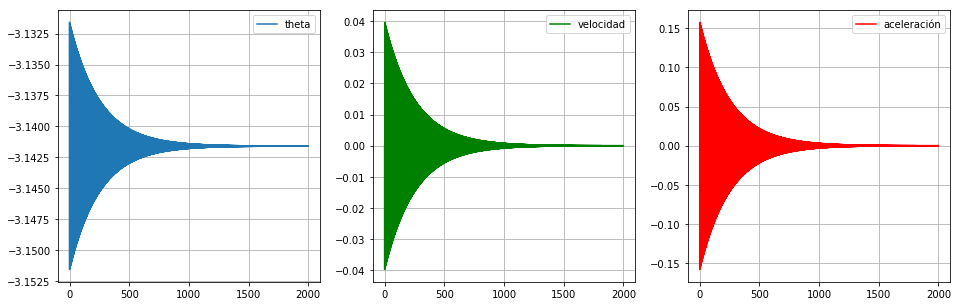
\includegraphics{output_8_0.png}

A pesar de que el modelo no considera ningún tipo de amortiguamiento,
puede observarse cómo el sistema ``pierde energía''. Esto es debido a
que el análisis es discreto, y a lo largo de las iteraciones se acumula
un error cada vez que el péndulo llega a los extremos, produciendo un
efecto similar al de un amortiguamiento.

\hypertarget{definiciuxf3n-de-las-variables-linguuxedsticas-y-los-conjuntos-borrosos-de-entrada}{%
\subsection{Definición de las variables linguísticas y los conjuntos
borrosos de
entrada}\label{definiciuxf3n-de-las-variables-linguuxedsticas-y-los-conjuntos-borrosos-de-entrada}}

Se elige como variables de entrada el ángulo \(\theta\) y la velocidad
angular. Ambos conjuntos borrosos pueden tomar valores \emph{MN}, muy
negativo, \emph{N}, negativo, \emph{Z}, cero, \emph{P}, positivo y
\emph{MP}, muy positivo.

\begin{Shaded}
\begin{Highlighting}[]
\ImportTok{from}\NormalTok{ numpy }\ImportTok{import}\NormalTok{ arange}
\ImportTok{from}\NormalTok{ matplotlib }\ImportTok{import}\NormalTok{ pyplot }\ImportTok{as}\NormalTok{ plt}
\ImportTok{from}\NormalTok{ math }\ImportTok{import}\NormalTok{ pi}
\ImportTok{from}\NormalTok{ fuzzy_logic }\ImportTok{import}\NormalTok{ generate_profile}

\NormalTok{T_STEP }\OperatorTok{=} \FloatTok{0.001}      \CommentTok{# [rad]}
\NormalTok{V_STEP }\OperatorTok{=} \FloatTok{0.005}      \CommentTok{# [rad/s]}
\NormalTok{A_STEP }\OperatorTok{=} \FloatTok{0.01}
\NormalTok{F_STEP }\OperatorTok{=} \FloatTok{0.05}

\NormalTok{theta }\OperatorTok{=}\NormalTok{ []}
\NormalTok{v }\OperatorTok{=}\NormalTok{ []}

\NormalTok{ang_vel }\OperatorTok{=} \DecValTok{15}
\NormalTok{force_mag }\OperatorTok{=} \DecValTok{10}

\NormalTok{theta.append(arange(}\OperatorTok{-}\DecValTok{2}\OperatorTok{*}\NormalTok{pi, }\DecValTok{2}\OperatorTok{*}\NormalTok{pi}\OperatorTok{+}\NormalTok{T_STEP, T_STEP))}
\NormalTok{v.append(arange(}\OperatorTok{-}\NormalTok{ang_vel, ang_vel}\OperatorTok{+}\NormalTok{V_STEP, V_STEP))}
\ControlFlowTok{for}\NormalTok{ i }\KeywordTok{in} \BuiltInTok{range}\NormalTok{(}\DecValTok{0}\NormalTok{, }\BuiltInTok{len}\NormalTok{(v[}\DecValTok{0}\NormalTok{])):}
\NormalTok{    v[}\DecValTok{0}\NormalTok{][i] }\OperatorTok{=} \BuiltInTok{round}\NormalTok{(v[}\DecValTok{0}\NormalTok{][i], }\DecValTok{3}\NormalTok{)}

\CommentTok{# Generación de conjuntos borrosos de entrada}

\CommentTok{# Conjunto borroso de theta:}
\NormalTok{theta.append(\{\})}
\NormalTok{theta[}\DecValTok{1}\NormalTok{][}\StringTok{'MN'}\NormalTok{] }\OperatorTok{=}\NormalTok{ generate_profile(}\OperatorTok{-}\NormalTok{pi}\OperatorTok{/}\DecValTok{4}\NormalTok{, theta[}\DecValTok{0}\NormalTok{], }\BuiltInTok{max}\OperatorTok{=-}\NormalTok{pi}\OperatorTok{/}\DecValTok{6}\NormalTok{)}
\NormalTok{theta[}\DecValTok{1}\NormalTok{][}\StringTok{'N'}\NormalTok{] }\OperatorTok{=}\NormalTok{ generate_profile(}\OperatorTok{-}\NormalTok{pi}\OperatorTok{/}\DecValTok{9}\NormalTok{, theta[}\DecValTok{0}\NormalTok{], }\BuiltInTok{min}\OperatorTok{=-}\NormalTok{pi}\OperatorTok{/}\DecValTok{3}\NormalTok{, }\BuiltInTok{max}\OperatorTok{=}\DecValTok{0}\NormalTok{)}
\NormalTok{theta[}\DecValTok{1}\NormalTok{][}\StringTok{'Z'}\NormalTok{] }\OperatorTok{=}\NormalTok{ generate_profile(}\DecValTok{0}\NormalTok{, theta[}\DecValTok{0}\NormalTok{], }\BuiltInTok{min}\OperatorTok{=-}\NormalTok{pi}\OperatorTok{/}\DecValTok{6}\NormalTok{, }\BuiltInTok{max}\OperatorTok{=}\NormalTok{pi}\OperatorTok{/}\DecValTok{6}\NormalTok{)}
\NormalTok{theta[}\DecValTok{1}\NormalTok{][}\StringTok{'P'}\NormalTok{] }\OperatorTok{=}\NormalTok{ generate_profile(pi}\OperatorTok{/}\DecValTok{9}\NormalTok{, theta[}\DecValTok{0}\NormalTok{], }\BuiltInTok{min}\OperatorTok{=}\DecValTok{0}\NormalTok{, }\BuiltInTok{max}\OperatorTok{=}\NormalTok{pi}\OperatorTok{/}\DecValTok{3}\NormalTok{)}
\NormalTok{theta[}\DecValTok{1}\NormalTok{][}\StringTok{'MP'}\NormalTok{] }\OperatorTok{=}\NormalTok{ generate_profile(pi}\OperatorTok{/}\DecValTok{4}\NormalTok{, theta[}\DecValTok{0}\NormalTok{], }\BuiltInTok{min}\OperatorTok{=}\NormalTok{pi}\OperatorTok{/}\DecValTok{6}\NormalTok{)}

\CommentTok{# Conjunto borroso de velocidad angular:}
\NormalTok{v.append(\{\})}
\NormalTok{v[}\DecValTok{1}\NormalTok{][}\StringTok{'MN'}\NormalTok{] }\OperatorTok{=}\NormalTok{ generate_profile(}\OperatorTok{-}\DecValTok{9}\NormalTok{, v[}\DecValTok{0}\NormalTok{], }\BuiltInTok{max}\OperatorTok{=-}\FloatTok{3.75}\NormalTok{)}
\NormalTok{v[}\DecValTok{1}\NormalTok{][}\StringTok{'N'}\NormalTok{] }\OperatorTok{=}\NormalTok{ generate_profile(}\OperatorTok{-}\FloatTok{3.5}\NormalTok{, v[}\DecValTok{0}\NormalTok{], }\BuiltInTok{min}\OperatorTok{=-}\FloatTok{6.5}\NormalTok{, }\BuiltInTok{max}\OperatorTok{=-}\FloatTok{0.03}\OperatorTok{*}\NormalTok{pi)}
\NormalTok{v[}\DecValTok{1}\NormalTok{][}\StringTok{'Z'}\NormalTok{] }\OperatorTok{=}\NormalTok{ generate_profile(}\DecValTok{0}\NormalTok{, v[}\DecValTok{0}\NormalTok{], }\BuiltInTok{min}\OperatorTok{=-}\DecValTok{3}\NormalTok{, }\BuiltInTok{max}\OperatorTok{=}\DecValTok{3}\NormalTok{)}
\NormalTok{v[}\DecValTok{1}\NormalTok{][}\StringTok{'P'}\NormalTok{] }\OperatorTok{=}\NormalTok{ generate_profile(}\FloatTok{3.5}\NormalTok{, v[}\DecValTok{0}\NormalTok{], }\BuiltInTok{min}\OperatorTok{=}\FloatTok{0.03}\OperatorTok{*}\NormalTok{pi, }\BuiltInTok{max}\OperatorTok{=}\FloatTok{6.5}\NormalTok{)}
\NormalTok{v[}\DecValTok{1}\NormalTok{][}\StringTok{'MP'}\NormalTok{] }\OperatorTok{=}\NormalTok{ generate_profile(}\DecValTok{9}\NormalTok{, v[}\DecValTok{0}\NormalTok{], }\BuiltInTok{min}\OperatorTok{=}\FloatTok{3.75}\NormalTok{)}
\end{Highlighting}
\end{Shaded}

Obteniendose los siguientes conjuntos borrosos para cada variable:

\begin{Shaded}
\begin{Highlighting}[]
\NormalTok{fig, (ax0, ax1) }\OperatorTok{=}\NormalTok{ plt.subplots(}\DecValTok{1}\NormalTok{, }\DecValTok{2}\NormalTok{, figsize}\OperatorTok{=}\NormalTok{(}\DecValTok{16}\NormalTok{, }\DecValTok{5}\NormalTok{))}
\ControlFlowTok{for}\NormalTok{ i }\KeywordTok{in}\NormalTok{ theta[}\DecValTok{1}\NormalTok{].values():}
\NormalTok{    ax0.plot(theta[}\DecValTok{0}\NormalTok{], i, label}\OperatorTok{=}\NormalTok{i)}
\NormalTok{ax0.grid()}
\NormalTok{ax0.set_xlim(}\OperatorTok{-}\FloatTok{2.5}\NormalTok{, }\FloatTok{2.5}\NormalTok{)}

\ControlFlowTok{for}\NormalTok{ i }\KeywordTok{in}\NormalTok{ v[}\DecValTok{1}\NormalTok{].values():}
\NormalTok{    ax1.plot(v[}\DecValTok{0}\NormalTok{], i, label}\OperatorTok{=}\NormalTok{i)}
\NormalTok{ax1.grid()}

\NormalTok{plt.show()}
\end{Highlighting}
\end{Shaded}

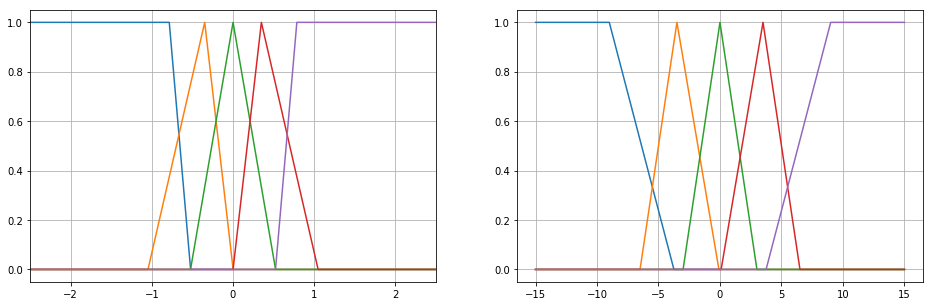
\includegraphics{output_14_0.png}

\hypertarget{definiciuxf3n-de-las-variable-linguuxedsticas-y-los-conjuntos-borrosos-de-salida}{%
\subsection{Definición de las variable linguísticas y los conjuntos
borrosos de
salida}\label{definiciuxf3n-de-las-variable-linguuxedsticas-y-los-conjuntos-borrosos-de-salida}}

Se elige como variable de salida del sistema la fuerza de acción
\emph{F} sobre el carro (base del péndulo invertido). Los diferentes
conjuntos se denominan igual, solo cambia el rango de valores reales que
puede tomar:

\begin{Shaded}
\begin{Highlighting}[]
\NormalTok{F }\OperatorTok{=}\NormalTok{ []}
\NormalTok{F.append(arange(}\OperatorTok{-}\DecValTok{7}\OperatorTok{*}\NormalTok{force_mag, }\DecValTok{7}\OperatorTok{*}\NormalTok{force_mag}\OperatorTok{+}\NormalTok{F_STEP, F_STEP))}

\CommentTok{# Generación de conjuntos borrosos de salida}
\NormalTok{F.append(\{\})}
\NormalTok{F[}\DecValTok{1}\NormalTok{][}\StringTok{'MN'}\NormalTok{] }\OperatorTok{=}\NormalTok{ generate_profile(}\OperatorTok{-}\DecValTok{5}\OperatorTok{*}\NormalTok{force_mag, F[}\DecValTok{0}\NormalTok{], }\BuiltInTok{max}\OperatorTok{=-}\FloatTok{3.5}\OperatorTok{*}\NormalTok{force_mag)}
\NormalTok{F[}\DecValTok{1}\NormalTok{][}\StringTok{'N'}\NormalTok{] }\OperatorTok{=}\NormalTok{ generate_profile(}\OperatorTok{-}\FloatTok{1.25}\OperatorTok{*}\NormalTok{force_mag, F[}\DecValTok{0}\NormalTok{], }\BuiltInTok{min}\OperatorTok{=-}\FloatTok{3.75}\OperatorTok{*}\NormalTok{force_mag, }\BuiltInTok{max}\OperatorTok{=}\DecValTok{0}\NormalTok{)}
\NormalTok{F[}\DecValTok{1}\NormalTok{][}\StringTok{'Z'}\NormalTok{] }\OperatorTok{=}\NormalTok{ generate_profile(}\DecValTok{0}\NormalTok{, F[}\DecValTok{0}\NormalTok{], }\BuiltInTok{min}\OperatorTok{=-}\FloatTok{1.5}\OperatorTok{*}\NormalTok{force_mag, }\BuiltInTok{max}\OperatorTok{=}\FloatTok{1.5}\OperatorTok{*}\NormalTok{force_mag)}
\NormalTok{F[}\DecValTok{1}\NormalTok{][}\StringTok{'P'}\NormalTok{] }\OperatorTok{=}\NormalTok{ generate_profile(}\FloatTok{1.25}\OperatorTok{*}\NormalTok{force_mag, F[}\DecValTok{0}\NormalTok{], }\BuiltInTok{min}\OperatorTok{=}\DecValTok{0}\NormalTok{, }\BuiltInTok{max}\OperatorTok{=}\FloatTok{3.75}\OperatorTok{*}\NormalTok{force_mag)}
\NormalTok{F[}\DecValTok{1}\NormalTok{][}\StringTok{'MP'}\NormalTok{] }\OperatorTok{=}\NormalTok{ generate_profile(}\DecValTok{5}\OperatorTok{*}\NormalTok{force_mag, F[}\DecValTok{0}\NormalTok{], }\BuiltInTok{min}\OperatorTok{=}\FloatTok{3.5}\OperatorTok{*}\NormalTok{force_mag)}
\end{Highlighting}
\end{Shaded}

Obteniendose los siguientes conjuntos borrosos para la variable F:

\begin{Shaded}
\begin{Highlighting}[]
\ControlFlowTok{for}\NormalTok{ i }\KeywordTok{in}\NormalTok{ theta[}\DecValTok{1}\NormalTok{]:}
\NormalTok{    plt.plot(F[}\DecValTok{0}\NormalTok{], F[}\DecValTok{1}\NormalTok{][i], label}\OperatorTok{=}\NormalTok{i)}
\NormalTok{plt.grid()}
\NormalTok{plt.legend(loc}\OperatorTok{=}\StringTok{"upper right"}\NormalTok{)}
\end{Highlighting}
\end{Shaded}

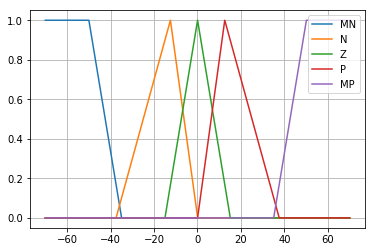
\includegraphics{output_19_1.png}

\hypertarget{implementaciuxf3n-de-la-inferencia-borrosa-mediante-base-de-reglas-tipo-if-then}{%
\subsection{Implementación de la inferencia borrosa mediante base de
reglas tipo
if-then}\label{implementaciuxf3n-de-la-inferencia-borrosa-mediante-base-de-reglas-tipo-if-then}}

Las base de reglas que se estableció para la inferencia borrosa se
expone en la siguiente tabla:

\begin{verbatim}
|    | MN | N  | Z  | P  | MP |
| -- | -- | -- | -- | -- | -- |
| MN | MN | MN | MN | N  | Z  |
| N  | MN | MN | N  | Z  | P  |
| Z  | MN | N  | Z  | P  | MP |
| P  | N  | Z  | P  | MP | MP |
| MP | Z  | P  | MP | MP | MP |
\end{verbatim}

la cual está implementada en python como un diccionario de diccionarios.
Esto debe leerse con la primera key del diccionario como el conjunto de
theta y cada key dentro de el diccionario de theta como los conjuntos de
theta punto. El valor resultante es un string que caracteriza el
conjunto borroso de F. Por ejemplo, R{[}`Z'{]}{[}`MP'{]} == `MP' lo que
significa que si theta es cero y theta punto es muy positiva entonces la
fuerza debe ser muy positiva

\begin{Shaded}
\begin{Highlighting}[]
\NormalTok{R }\OperatorTok{=}\NormalTok{ \{}
    \StringTok{'MN'}\NormalTok{: \{}\StringTok{'MN'}\NormalTok{: }\StringTok{'MN'}\NormalTok{, }\StringTok{'N'}\NormalTok{: }\StringTok{'MN'}\NormalTok{, }\StringTok{'Z'}\NormalTok{: }\StringTok{'MN'}\NormalTok{, }\StringTok{'P'}\NormalTok{: }\StringTok{'N'}\NormalTok{, }\StringTok{'MP'}\NormalTok{: }\StringTok{'Z'}\NormalTok{\},}
    \StringTok{'N'}\NormalTok{: \{}\StringTok{'MN'}\NormalTok{: }\StringTok{'MN'}\NormalTok{, }\StringTok{'N'}\NormalTok{: }\StringTok{'MN'}\NormalTok{, }\StringTok{'Z'}\NormalTok{: }\StringTok{'N'}\NormalTok{, }\StringTok{'P'}\NormalTok{: }\StringTok{'Z'}\NormalTok{, }\StringTok{'MP'}\NormalTok{: }\StringTok{'P'}\NormalTok{\},}
    \StringTok{'Z'}\NormalTok{: \{}\StringTok{'MN'}\NormalTok{: }\StringTok{'MN'}\NormalTok{, }\StringTok{'N'}\NormalTok{: }\StringTok{'N'}\NormalTok{, }\StringTok{'Z'}\NormalTok{: }\StringTok{'Z'}\NormalTok{, }\StringTok{'P'}\NormalTok{: }\StringTok{'P'}\NormalTok{, }\StringTok{'MP'}\NormalTok{: }\StringTok{'MP'}\NormalTok{\},}
    \StringTok{'P'}\NormalTok{: \{}\StringTok{'MN'}\NormalTok{: }\StringTok{'N'}\NormalTok{, }\StringTok{'N'}\NormalTok{: }\StringTok{'Z'}\NormalTok{, }\StringTok{'Z'}\NormalTok{: }\StringTok{'P'}\NormalTok{, }\StringTok{'P'}\NormalTok{: }\StringTok{'MP'}\NormalTok{, }\StringTok{'MP'}\NormalTok{: }\StringTok{'MP'}\NormalTok{\},}
    \StringTok{'MP'}\NormalTok{: \{}\StringTok{'MN'}\NormalTok{: }\StringTok{'Z'}\NormalTok{, }\StringTok{'N'}\NormalTok{: }\StringTok{'P'}\NormalTok{, }\StringTok{'Z'}\NormalTok{: }\StringTok{'MP'}\NormalTok{, }\StringTok{'P'}\NormalTok{: }\StringTok{'MP'}\NormalTok{, }\StringTok{'MP'}\NormalTok{: }\StringTok{'MP'}\NormalTok{\}}
\NormalTok{    \}}
\end{Highlighting}
\end{Shaded}

\hypertarget{obtenciuxf3n-de-la-fuerza-dadas-las-condiciones-iniciales}{%
\subsection{Obtención de la fuerza dadas las condiciones
iniciales}\label{obtenciuxf3n-de-la-fuerza-dadas-las-condiciones-iniciales}}

Dadas ciertas condiciones iniciales probamos lo que hace el controlador
difuso para un delta\_t. Primero obtenemos los valores de pertenencia de
las condiciones iniciales a cada conjunto borroso de su variable
lingüística.

\begin{Shaded}
\begin{Highlighting}[]
\ImportTok{from}\NormalTok{ fuzzy_logic }\ImportTok{import}\NormalTok{ fuzzifier, defuzzifier}
\ImportTok{from}\NormalTok{ numpy }\ImportTok{import}\NormalTok{ zeros}

\NormalTok{cond_inic }\OperatorTok{=}\NormalTok{ [pi}\OperatorTok{/}\DecValTok{6}\NormalTok{, pi}\OperatorTok{/}\DecValTok{4}\NormalTok{]}

\NormalTok{value }\OperatorTok{=}\NormalTok{ zeros(}\DecValTok{3}\NormalTok{)}
\NormalTok{value[}\DecValTok{0}\NormalTok{] }\OperatorTok{=}\NormalTok{ cond_inic[}\DecValTok{0}\NormalTok{]}
\NormalTok{value[}\DecValTok{1}\NormalTok{] }\OperatorTok{=}\NormalTok{ cond_inic[}\DecValTok{1}\NormalTok{]}
\NormalTok{value[}\DecValTok{2}\NormalTok{] }\OperatorTok{=} \DecValTok{0}

\NormalTok{Force }\OperatorTok{=} \DecValTok{0}

\NormalTok{mu_theta }\OperatorTok{=}\NormalTok{ fuzzifier(value[}\DecValTok{0}\NormalTok{], theta)}
\NormalTok{mu_thetadot }\OperatorTok{=}\NormalTok{ fuzzifier(value[}\DecValTok{1}\NormalTok{], v)}

\BuiltInTok{print}\NormalTok{(mu_theta)}
\BuiltInTok{print}\NormalTok{(mu_thetadot)}
\end{Highlighting}
\end{Shaded}

\begin{verbatim}
{'MN': 0, 'N': 0, 'Z': 0.0, 'P': 0.7507163323782235, 'MP': 0.0}
{'MN': 0, 'N': 0, 'Z': 0.7366666666666667, 'P': 0.20411160058737152, 'MP': 0}
\end{verbatim}

Luego se realiza el cálculo de los antecedentes de cada regla en las que
intervienen los valores no nulos de pertenencia que acabamos de
calcular.

\begin{Shaded}
\begin{Highlighting}[]
\NormalTok{v_antec }\OperatorTok{=}\NormalTok{ \{}\StringTok{'MN'}\NormalTok{: }\DecValTok{0}\NormalTok{, }\StringTok{'N'}\NormalTok{: }\DecValTok{0}\NormalTok{, }\StringTok{'Z'}\NormalTok{:}\DecValTok{0}\NormalTok{, }\StringTok{'P'}\NormalTok{: }\DecValTok{0}\NormalTok{, }\StringTok{'MP'}\NormalTok{: }\DecValTok{0}\NormalTok{\}}

\ControlFlowTok{for}\NormalTok{ theta_r }\KeywordTok{in}\NormalTok{ R.keys():}
    \ControlFlowTok{for}\NormalTok{ thetadot_r }\KeywordTok{in}\NormalTok{ R[theta_r].keys():}
        \ControlFlowTok{if}\NormalTok{ (mu_thetadot[thetadot_r] }\OperatorTok{==} \DecValTok{0}\NormalTok{) }\KeywordTok{or}\NormalTok{ (mu_theta[theta_r] }\OperatorTok{==} \DecValTok{0}\NormalTok{): }
            \ControlFlowTok{continue}

\NormalTok{        antec }\OperatorTok{=} \BuiltInTok{min}\NormalTok{(mu_theta[theta_r], mu_thetadot[thetadot_r])}

        \ControlFlowTok{if}\NormalTok{ (antec }\OperatorTok{>}\NormalTok{ v_antec[R[theta_r][thetadot_r]]):}
\NormalTok{            v_antec[R[theta_r][thetadot_r]] }\OperatorTok{=}\NormalTok{ antec}
\end{Highlighting}
\end{Shaded}

Posteriormente ealizamos la implicación de cada regla. Esto genera el
truncamiento de los conjuntos borrosos de salida de la variable fuerza.
Finalmente encontramos el valor nítido de fuerza usando el
desborrosificador de centro de gravedad conjunto truncado.

\begin{Shaded}
\begin{Highlighting}[]
\CommentTok{# Implicación/truncado de conjuntos de salida:    }
\NormalTok{F_out }\OperatorTok{=}\NormalTok{ zeros(}\BuiltInTok{len}\NormalTok{(F[}\DecValTok{0}\NormalTok{]))}

\ControlFlowTok{for}\NormalTok{ i }\KeywordTok{in}\NormalTok{ F[}\DecValTok{1}\NormalTok{].keys():}
    \ControlFlowTok{for}\NormalTok{ j }\KeywordTok{in} \BuiltInTok{range}\NormalTok{(}\DecValTok{0}\NormalTok{, }\BuiltInTok{len}\NormalTok{(F[}\DecValTok{0}\NormalTok{])):}

\NormalTok{        min_temp }\OperatorTok{=} \BuiltInTok{min}\NormalTok{(F[}\DecValTok{1}\NormalTok{][i][j], v_antec[i])}

        \ControlFlowTok{if}\NormalTok{ (min_temp }\OperatorTok{>}\NormalTok{ F_out[j]):}
\NormalTok{            F_out[j] }\OperatorTok{=}\NormalTok{ min_temp            }

\NormalTok{plt.plot(F[}\DecValTok{0}\NormalTok{], F_out)}
\NormalTok{force }\OperatorTok{=}\NormalTok{ defuzzifier(F_out, F[}\DecValTok{0}\NormalTok{])}

\BuiltInTok{print}\NormalTok{(}\StringTok{"fuerza="}\NormalTok{,force)}
\end{Highlighting}
\end{Shaded}

\begin{verbatim}
fuerza= 27.149999999994478
\end{verbatim}

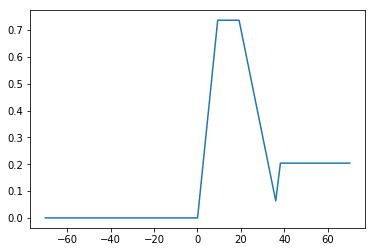
\includegraphics{output_29_1.png}

\hypertarget{controlador-difuso}{%
\subsection{Controlador difuso}\label{controlador-difuso}}

Luego de verificar el funcionamiento del algoritmo difuso pasamos a
realizar un control de posición el cual se basa en ejecutar lo antes
explicado iterativamente y calculando las nuevas posiciones y
velocidades angulares con el modelo del péndulo invertido también ya
descripto.

\begin{Shaded}
\begin{Highlighting}[]
\ImportTok{from}\NormalTok{ fuzzy_logic }\ImportTok{import}\NormalTok{ fuzzy_control}
\ImportTok{from}\NormalTok{ math }\ImportTok{import}\NormalTok{ pi}
\ImportTok{from}\NormalTok{ numpy }\ImportTok{import}\NormalTok{ zeros}

\NormalTok{cond_inic }\OperatorTok{=}\NormalTok{ [pi}\OperatorTok{/}\DecValTok{4}\NormalTok{, pi}\OperatorTok{/}\DecValTok{8}\NormalTok{]}

\NormalTok{x }\OperatorTok{=}\NormalTok{ zeros(}\DecValTok{3}\NormalTok{)}
\NormalTok{x[}\DecValTok{0}\NormalTok{] }\OperatorTok{=}\NormalTok{ cond_inic[}\DecValTok{0}\NormalTok{]}
\NormalTok{x[}\DecValTok{1}\NormalTok{] }\OperatorTok{=}\NormalTok{ cond_inic[}\DecValTok{1}\NormalTok{]}
\NormalTok{x[}\DecValTok{2}\NormalTok{] }\OperatorTok{=} \DecValTok{0}

\NormalTok{pos }\OperatorTok{=}\NormalTok{ []}
\NormalTok{vel }\OperatorTok{=}\NormalTok{ []}
\NormalTok{acel }\OperatorTok{=}\NormalTok{ []}
\NormalTok{time }\OperatorTok{=}\NormalTok{ []}

\NormalTok{Force }\OperatorTok{=} \DecValTok{0}
\NormalTok{force_hist }\OperatorTok{=}\NormalTok{ []}
\NormalTok{t }\OperatorTok{=} \DecValTok{0}
\NormalTok{dt }\OperatorTok{=} \FloatTok{0.05}


\ControlFlowTok{while}\NormalTok{(t }\OperatorTok{<} \DecValTok{8}\NormalTok{):}

\NormalTok{    x }\OperatorTok{=}\NormalTok{ update(x, dt, Force)}

\NormalTok{    pos.append(x[}\DecValTok{0}\NormalTok{])}
\NormalTok{    vel.append(x[}\DecValTok{1}\NormalTok{])}
\NormalTok{    acel.append(x[}\DecValTok{2}\NormalTok{])}

\NormalTok{    Force }\OperatorTok{=}\NormalTok{ fuzzy_control([x[}\DecValTok{0}\NormalTok{], x[}\DecValTok{1}\NormalTok{]], theta, v, R, F)}
\NormalTok{    force_hist.append(Force)}
\NormalTok{    time.append(t)}

\NormalTok{    t }\OperatorTok{+=}\NormalTok{ dt}
\end{Highlighting}
\end{Shaded}

Para un ángulo inicial de pi/4 rad y una velocidad angular inicial de
pi/8 rad/s obtenemos estas respuestas de posición, velocidad y
aceleración angulares.

\begin{Shaded}
\begin{Highlighting}[]
\NormalTok{fig, (ax0, ax1, ax2) }\OperatorTok{=}\NormalTok{ plt.subplots(}\DecValTok{1}\NormalTok{, }\DecValTok{3}\NormalTok{, figsize}\OperatorTok{=}\NormalTok{(}\DecValTok{16}\NormalTok{, }\DecValTok{5}\NormalTok{))}
\NormalTok{ax0.plot(time, pos)}
\NormalTok{ax0.grid()}
\NormalTok{ax1.plot(time, vel)}
\NormalTok{ax1.grid()}
\NormalTok{ax2.plot(time, acel)}
\NormalTok{ax2.grid()}
\end{Highlighting}
\end{Shaded}

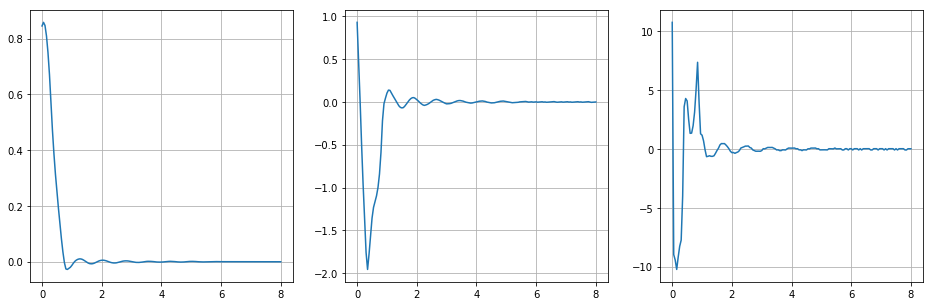
\includegraphics{output_34_0.png}

Además el perfil de fuerzas es el siguiente

\begin{Shaded}
\begin{Highlighting}[]
\NormalTok{plt.plot(time, force_hist)}
\NormalTok{plt.show()}
\end{Highlighting}
\end{Shaded}

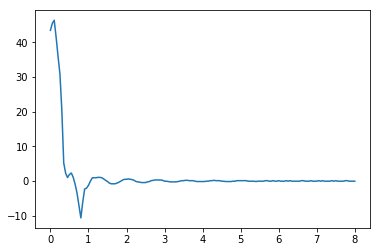
\includegraphics{output_36_0.png}

\hypertarget{levantar-el-puxe9ndulo}{%
\subsection{Levantar el péndulo}\label{levantar-el-puxe9ndulo}}

También existe la posibilidad de levantar el péndulo desde una posición
inicial vertical, hacia abajo (pi radianes).

\begin{Shaded}
\begin{Highlighting}[]
\ImportTok{from}\NormalTok{ fuzzy_logic }\ImportTok{import}\NormalTok{ fuzzy_control}
\ImportTok{from}\NormalTok{ math }\ImportTok{import}\NormalTok{ pi}
\ImportTok{from}\NormalTok{ numpy }\ImportTok{import}\NormalTok{ zeros}

\NormalTok{cond_inic }\OperatorTok{=}\NormalTok{ [pi, }\DecValTok{0}\NormalTok{]}

\NormalTok{x }\OperatorTok{=}\NormalTok{ zeros(}\DecValTok{3}\NormalTok{)}
\NormalTok{x[}\DecValTok{0}\NormalTok{] }\OperatorTok{=}\NormalTok{ cond_inic[}\DecValTok{0}\NormalTok{]}
\NormalTok{x[}\DecValTok{1}\NormalTok{] }\OperatorTok{=}\NormalTok{ cond_inic[}\DecValTok{1}\NormalTok{]}
\NormalTok{x[}\DecValTok{2}\NormalTok{] }\OperatorTok{=} \DecValTok{0}

\NormalTok{pos }\OperatorTok{=}\NormalTok{ []}
\NormalTok{vel }\OperatorTok{=}\NormalTok{ []}
\NormalTok{acel }\OperatorTok{=}\NormalTok{ []}
\NormalTok{time }\OperatorTok{=}\NormalTok{ []}

\NormalTok{Force }\OperatorTok{=} \DecValTok{0}
\NormalTok{force_hist }\OperatorTok{=}\NormalTok{ []}
\NormalTok{t }\OperatorTok{=} \DecValTok{0}
\NormalTok{dt }\OperatorTok{=} \FloatTok{0.05}


\ControlFlowTok{while}\NormalTok{(t }\OperatorTok{<} \DecValTok{8}\NormalTok{):}

\NormalTok{    x }\OperatorTok{=}\NormalTok{ update(x, dt, Force)}

\NormalTok{    pos.append(x[}\DecValTok{0}\NormalTok{])}
\NormalTok{    vel.append(x[}\DecValTok{1}\NormalTok{])}
\NormalTok{    acel.append(x[}\DecValTok{2}\NormalTok{])}

\NormalTok{    Force }\OperatorTok{=}\NormalTok{ fuzzy_control([x[}\DecValTok{0}\NormalTok{], x[}\DecValTok{1}\NormalTok{]], theta, v, R, F)}
\NormalTok{    force_hist.append(Force)}
\NormalTok{    time.append(t)}

\NormalTok{    t }\OperatorTok{+=}\NormalTok{ dt}
\end{Highlighting}
\end{Shaded}

Y las curvas obtenidas de ángulo, velocidad, aceleración y fuerza son
las siguientes

\begin{Shaded}
\begin{Highlighting}[]
\NormalTok{fig, (ax0, ax1, ax2) }\OperatorTok{=}\NormalTok{ plt.subplots(}\DecValTok{1}\NormalTok{, }\DecValTok{3}\NormalTok{, figsize}\OperatorTok{=}\NormalTok{(}\DecValTok{16}\NormalTok{, }\DecValTok{5}\NormalTok{))}
\NormalTok{ax0.plot(time, pos)}
\NormalTok{ax0.grid()}
\NormalTok{ax1.plot(time, vel)}
\NormalTok{ax1.grid()}
\NormalTok{ax2.plot(time, acel)}
\NormalTok{ax2.grid()}
\end{Highlighting}
\end{Shaded}

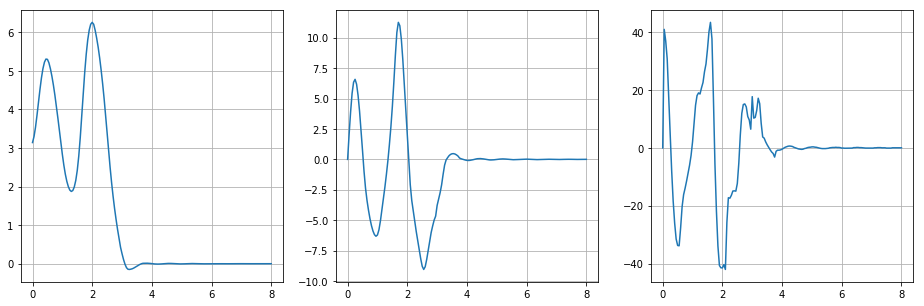
\includegraphics{output_41_0.png}

\begin{Shaded}
\begin{Highlighting}[]
\NormalTok{plt.plot(time, force_hist)}
\NormalTok{plt.show()}
\end{Highlighting}
\end{Shaded}

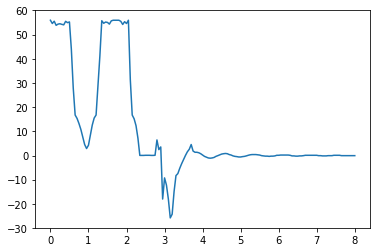
\includegraphics{output_42_0.png}

\begin{Shaded}
\begin{Highlighting}[]

\end{Highlighting}
\end{Shaded}

\hypertarget{ejercicios-de-planificaciuxf3n-con-fast-downward}{%
\section{Ejercicios de planificación con Fast
Downward}\label{ejercicios-de-planificaciuxf3n-con-fast-downward}}

\hypertarget{dominio-de-transporte-auxe9reo-de-cargas}{%
\subsection{Dominio de transporte aéreo de
cargas}\label{dominio-de-transporte-auxe9reo-de-cargas}}

La consigna consiste en modelar en PDDl el dominio de transporte aéreo
de cargas y definir algunas instancias del problema para luego encontrar
soluciones con el planificador Fast Downward.

El modelado del problema fue basado en el ejemplo de planificación visto
en clase.

En el archivo \href{planning/domain3a.pddl}{domain3a.pddl} se definió el
dominio del problema, con los predicados \emph{LOAD}, \emph{PLANE} y
\emph{AIRPORT} para definir variables y \emph{in} y \emph{at} para
definir estados de las variables. Las acciones definidas fueron:

\begin{itemize}
\tightlist
\item
  \emph{fly}, parámetros \emph{p}, \emph{from} y \emph{to}. Acción en la
  que el avión \emph{p} vuela del aeropuerto \emph{from} al aeropuerto
  \emph{to}.
\item
  \emph{load}, parámetros \emph{c}, \emph{p} y \emph{a}. Acción de
  cargar \emph{c}, en el avión \emph{p}, en el aeropuerto \emph{a}.
\item
  \emph{unload}, parámetros \emph{c}, \emph{p} y \emph{a}. Acción de
  descargar \emph{c}, en el avión \emph{p}, en el aeropuerto \emph{a}.
\end{itemize}

En el archivo \href{planning/task3a.pddl}{task3a.pddl} se dan las
condiciones iniciales del problema en específico, instanciando dos
aviones, dos aeropuertos y dos cargas diferentes; y el estado objetivo
donde las cargas deben estar en los aeropuertos diferentes al que
comienzan.

\hypertarget{soluciuxf3n}{%
\subsubsection{Solución}\label{soluciuxf3n}}

\begin{verbatim}
 (load c2 p2 jfk)
 (fly p2 jfk sf0)
 (unload c2 p2 sf0)
 (load c1 p2 sf0)
 (fly p2 sf0 jfk)
 (unload c1 p2 jfk)
 ; cost = 6 (unit cost)
\end{verbatim}

\hypertarget{dificultades}{%
\subsubsection{Dificultades}\label{dificultades}}

No se pudo lograr que el planificador logre paralelizar el problema para
que contemple en la solución el uso de ambos aviones (reduciendo el
costo temporal). Se concluyó que dado que el planificador Fast Downward
solo soporta hasta PDDL 2, no se puede realizar esto en dicha versión
del lenguaje.

\hypertarget{planificaciuxf3n-de-procesos-asistida-por-computadora}{%
\subsection{Planificación de Procesos Asistida por
Computadora}\label{planificaciuxf3n-de-procesos-asistida-por-computadora}}

La consigna consiste en modelar en PDDL y definir una instancia del
problema de planificación de Procesos Asistida por Computadora (CAPP,
Computer-Aided Process Planning).

En el archivo \href{planning/domain3b.pddl}{domain3b.pddl} se definió el
dominio del problema, con los predicados \emph{CUERPO},
\emph{HERRAMIENTA}, \emph{ARMARIO}, \emph{HUSILLO}, \emph{DIRECCIÓN},
\emph{AGUJERO} y \emph{RANURA} para definir variables y \emph{en} y
\emph{vinculo} (para relacionar un tipo de operación con determinada
herramienta) para definir estados de las variables. Las acciones
definidas fueron:

\begin{itemize}
\tightlist
\item
  \emph{cambio-herramienta}, parámetros \emph{h1}, \emph{h2}, \emph{a} y
  \emph{m}. Acción en la que se reemplaza las herramientas \emph{h1} y
  \emph{h2} que están en el armario \emph{a} y el husillo de la máquina
  \emph{m} respectivamente.
\item
  \emph{agujerear}, parámetros \emph{p}, \emph{h}, \emph{m} y \emph{a}.
  Acción de realizar un agujero tipo \emph{a} en el cuerpo \emph{p} con
  la herramienta \emph{h} en el husillo de la máquina \emph{m}.
\item
  \emph{fresar}, parámetros \emph{p}, \emph{h}, \emph{m} y \emph{r}.
  Acción de realizar una ranura tipo \emph{r} en el cuerpo \emph{p} con
  la herramienta \emph{h} en el husillo de la máquina \emph{m}.
\end{itemize}

En el archivo \href{planning/task3b.pddl}{task3b.pddl} se dan las
condiciones iniciales del problema en específico, instanciando tres
herramientas para realizar tres tipos de gujeros diferentes (brocas),
tres tipos de herramientas para realizar tres tipos de ranuras (fresas)
y la materia prima; y el estado objetivo donde ya se encuentra el
producto final con los tres agujeros y ranuras realizados.

\hypertarget{soluciuxf3n-1}{%
\subsubsection{Solución}\label{soluciuxf3n-1}}

\begin{verbatim}
(fresar p f1 m r1)
(cambio-herramienta b1 f1 a m)
(agujerear p b1 m h1)
(cambio-herramienta b2 b1 a m)
(agujerear p b2 m h2)
(cambio-herramienta b3 b2 a m)
(agujerear p b3 m h3)
(cambio-herramienta f2 b3 a m)
(fresar p f2 m r2)
(cambio-herramienta f3 f2 a m)
(fresar p f3 m r3)
; cost = 11 (unit cost)
\end{verbatim}

\hypertarget{dificulatades}{%
\subsubsection{Dificulatades}\label{dificulatades}}

Dado que el planificador Fast Downward soporta PDDL solo hasta segunda
versión, no se pudo implementar restricciones blandas de precedencia
entre las tareas, pero se expresaría de la siguiente manera:

\begin{verbatim}
(:goal
...
    (preference precendencia
        (sometime-after (en p r2) (en p r1))
        (sometime-after (en p h1) (en p r1))
    )

...
)
\end{verbatim}

Explicitando la preferencia de ejecución de dos tareas en un determinado
orden, y estableciendo un métrica de la forma:

\begin{verbatim}
(:metric (minimize (is-violated precedencia)))
\end{verbatim}

\end{document}
